\documentclass{article}
\usepackage{tikz, comment}
\usepackage{pifont}
\usepackage{fontspec}
\usetikzlibrary{arrows, decorations.markings, decorations.pathreplacing}
\begin{comment}
:Title: Not defined yet
:Tags: area using parametric equations,parametric integral formula;area under a curve;approximation by differentials;root;average rate of change, arc 
:Prob: 0.4155;0.4087;0.4007;0.3994;0.3944
:Author: Prof.Hu Ji-shan, HKUST
:Slug: No name yet

Description Here.........
\end{comment}
\begin{document}\centering

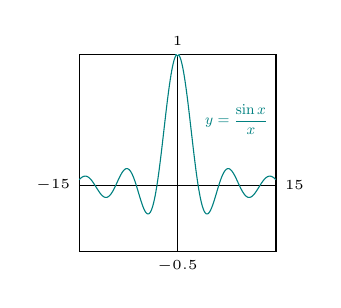
\begin{tikzpicture}[>=latex,xscale=0.25*10/30, yscale=0.25*10/1.5][font=\sf\small]

%\draw[xstep=1cm,ystep=1cm,color=gray!20] (-15, -0.5) grid (15, 1);

\draw[] (-15, 0) -- (15, 0);
\draw[] (0, -0.5) -- (0, 1);

\node[left] at (-15, 0) {\tiny$-15$};
\node[right] at (15, 0) {\tiny$15$};
\node[below] at (0, -0.5) {\tiny$-0.5$};
\node[above] at (0, 1) {\tiny$1$};

\clip[draw] (-15, -0.5) rectangle (15, 1);

\draw[teal, samples=200, smooth, domain=0.01:15, variable=\x]
plot ({\x}, {(sin(\x r))/(\x)});

\draw[teal, samples=200, smooth, domain=-0.01:-15, variable=\x]
plot ({\x}, {(sin(\x r))/(\x)});

\node[teal, scale=0.6] at (9, 0.5) {$\displaystyle y = \frac{\sin x}{x}$};

\draw[teal, fill=white, xscale=6, yscale=0.3] ({0/0.3}, {1/0.3}) circle(0.05);

\end{tikzpicture}\hskip 1cm
\end{document}